

\let\clearpage\relax


% \begin{table}
% 	\begin{minipage}{0.5\linewidth}
% 		\caption{Student Database}
% 		\label{table:student}
% 		\centering

% \begin{tabular}[t]{llc}
% %%%%%% Title row starts here
% % Temporary header Graph would be better! TBD
% \toprule
% \multicolumn{2}{l}{} & mIOU \\
% \midrule
% \multicolumn{2}{l}{Baseline} & 75.79 \\
% \multicolumn{2}{l}{Baseline + SDC} & 76.37 \\
% \multicolumn{2}{l}{Baseline + LID} & 76.37 \\
% \bottomrule
% \end{tabular}
% 	\end{minipage}\hfill
% 	\begin{minipage}{0.45\linewidth}
% 		\centering
% 		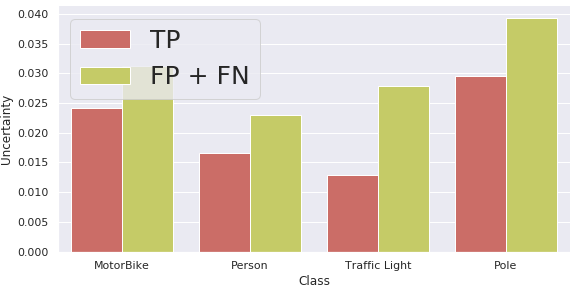
\includegraphics[width=1.0\linewidth]{figures/uncertainty.png}
% 		\captionof{figure}{2-D scatterplot of the Student Database}
% 		\label{ }
% 	\end{minipage}
% \end{table}
\begin{figure}\CenterFloatBoxes
\begin{floatrow}
\ffigbox[1.0\linewidth][]
{%
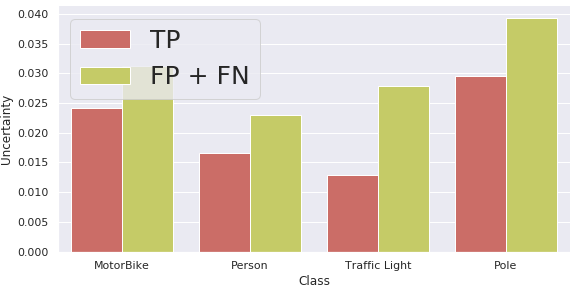
\includegraphics[height=0.4\linewidth]{figures/uncertainty.png}}
{%
\vspace{-0.3em}%
\caption{ Precision vs Recall plot showing uncertainty effectively captures noise in label generation.}\label{fig: figure-label}}
\killfloatstyle\ttabbox[\Xhsize]
{%
\begin{tabular}[b]{llc}
%%%%%% Title row starts here
% Temporary header Graph would be better! TBD
\toprule
\multicolumn{2}{l}{} & mIOU \\
\midrule
\multicolumn{2}{l}{Baseline} & 77.66 \\
\multicolumn{2}{l}{Baseline  + \cite{nvidia_cvpr19} ($\pm 3$)}+ RLL  & 77.24 \\
\multicolumn{2}{l}{Baseline + Ours($\pm 3$)}+ RLL  & 77.50 \\
\bottomrule
\end{tabular}%
}%
{\caption{ Addding a single propagated frame, and relaxed label loss (RLL)~\cite{nvidia_cvpr19} is ineffective.}\label{tab: table-label}}%
\end{floatrow}

% \caption{\small \emph{Left:} The sequence error for SVHN multi-digit recognition
% on crops of $64\times 64$ pixels (64px), and inflated crops of $128 \times 128$
% (128px) which include more background. \textsuperscript{*}The best reported
% result from \cite{Ba14} uses model averagin}
% % }}%
\vspace{-1em}
\end{figure}

% \begin{figure}
% \begin{floatrow}
% \capbtabbox{%
% \centering%
% \begin{tabular}[t]{llc}
% %%%%%% Title row starts here
% % Temporary header Graph would be better! TBD
% \toprule
% \multicolumn{2}{l}{} & mIOU \\
% \midrule
% \multicolumn{2}{l}{Baseline} & 75.79 \\
% \multicolumn{2}{l}{Baseline + SDC} & 76.37 \\
% \multicolumn{2}{l}{Baseline + LID} & 76.37 \\
% \bottomrule
% \end{tabular}
% }{%
%   \caption{This is the great table of asgard}%
% }%
% \ffigbox{%
% \centering%
% 				\label{fig:input-model}
% 				% \centering
% 				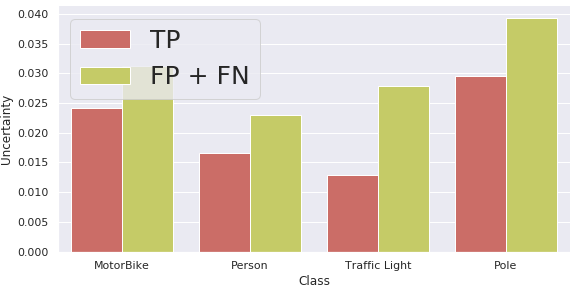
\includegraphics[width=0.5\linewidth]{figures/uncertainty.png}%
% }{%
%   \caption{A figure from asgard}%
% }%
% \end{floatrow}
% \end{figure}



% \begin{figure}[t]
% \begin{center}% \small
% % \setlength{\tabcolsep}{3pt}

% \label{table:svhn}
% 		\subfigure[b]{
% \begin{minipage}{0.45\textwidth}
% \centering
% \begin{tabular}[t]{llc}
% %%%%%% Title row starts here
% \\
% % Temporary header Graph would be better! TBD
% \toprule
% \multicolumn{2}{l}{} & mIOU \\
% \midrule
% \multicolumn{2}{l}{Baseline} & 75.79 \\
% \multicolumn{2}{l}{Baseline + SDC} & 76.37 \\
% \multicolumn{2}{l}{Baseline + LID} & 76.37 \\
% \bottomrule
% \end{tabular}
% \end{minipage}
% % }}%
% \caption{Corrected Evalutation of previous work\cite{nvidia_cvpr19}}
% }
% % \qquad\qquad \qquad\qquad
% % \hspace{2em}
% % \vtop{
% % \hfill
% % \hbox{
% % 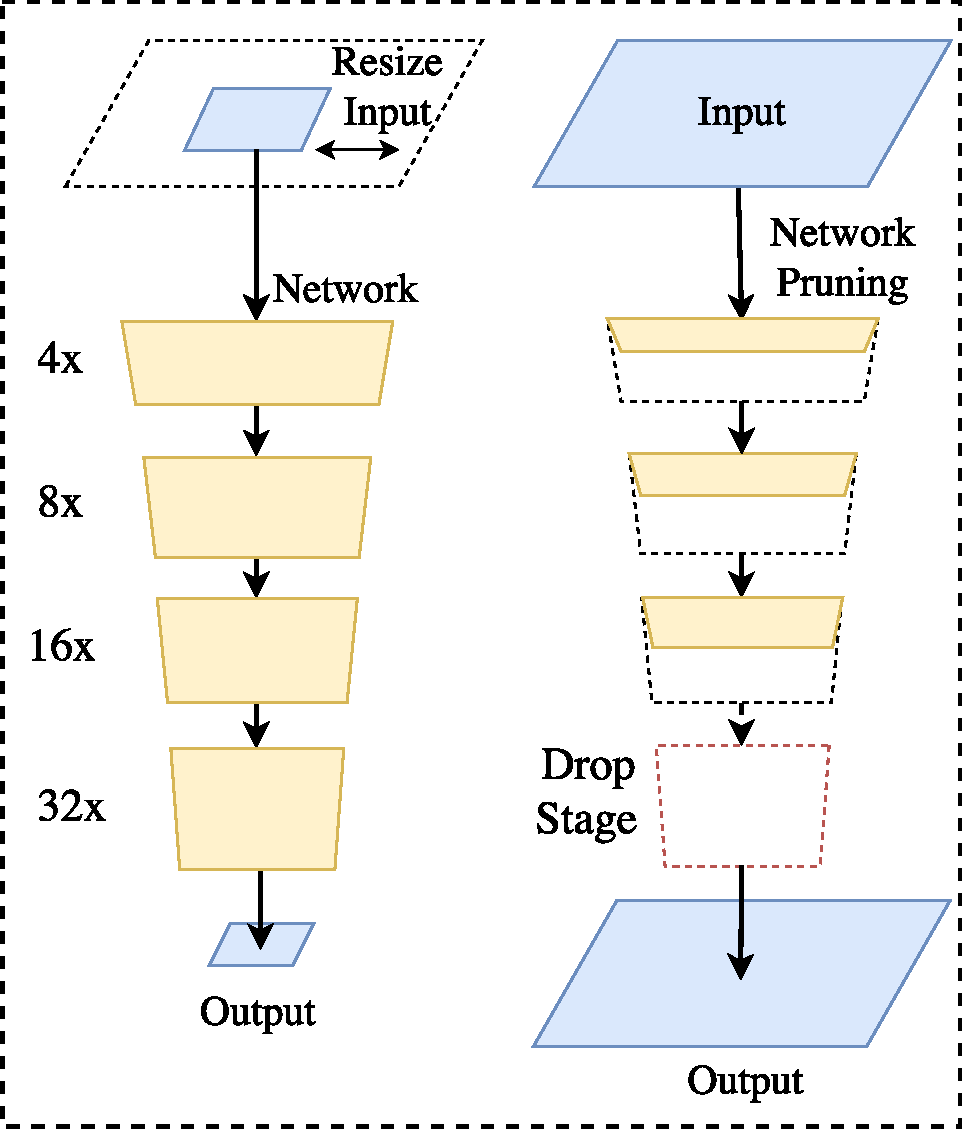
\includegraphics[width=0.6\textwidth]{figures/input_model.pdf}
% 		\subfigure[b]{
% \begin{minipage}{0.30\textwidth}
% \centering
% 				\label{fig:input-model}
% 				% \centering
% 				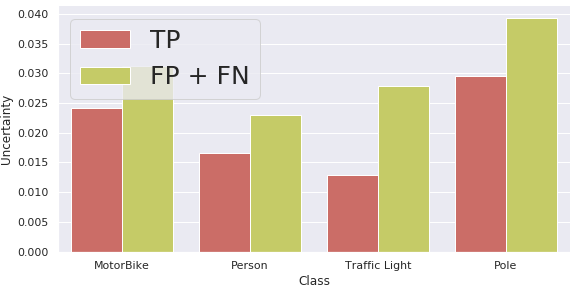
\includegraphics[width=1.0\linewidth]{figures/uncertainty.png}
% \end{minipage}
% \caption{Precision-Recall Curve}
% }

% \caption{\small \emph{Left:} The sequence error for SVHN multi-digit recognition
% on crops of $64\times 64$ pixels (64px), and inflated crops of $128 \times 128$
% (128px) which include more background. \textsuperscript{*}The best reported
% result from \cite{Ba14} uses model averagin}
% % }}%
% \end{center}
% 		\vspace{-2.0em}
% \end{figure}


\let\clearpage\relax
\begin{table}[t]
    \centering
    \caption{ We show the benefit of training with our pseudo-labels. We also show the benefit of modelling label uncertainty. In the above table,  $D_{\hat{L}seq}$ contains propagated labels and $D_{\hat{L}ps}$ contains pseudo-semantic labels (refer Section~\ref{subsec-alea}).
    }\label{tab_main_ablation}
    \begin{tabular}{llccc}
\toprule
\multicolumn{2}{c}{Dataset}& Cross Entropy & Aleatoric Uncertainty\cite{gal_main} & Ours: UAT \\
\midrule
\multicolumn{2}{l}{$D_L$} & 77.62 & 77.69 & - \\
\multicolumn{2}{l}{$D_L + D_{\hat{L}seq}$ }& 77.82 & 77.83 & 78.11 \\
\midrule
\multicolumn{2}{c}{$D_L + D_{\hat{L}seq} + D_{\hat{L}ps}$} & 78.45  & 78.52 & \textbf{78.58} \\
\bottomrule
    \end{tabular}
\end{table}
%Now, we present quantitative and qualitative evaluation of our proposed method. We break this section into two major parts: Evaluation of the propagation method, Evaluation of learning with propagated labels. Our experiments are performend on two widely adopted semantic segmentation datasets, Cityscapes and Apolloscape.

\subsection{Implementation Details}
For training the label refinement network $\mathtt{LRN}_\theta$, we utilize the dual-task loss~\cite{gated_iccv2019}.
For training semantic segmentation networks on manually annotated and generated labels we follow the training regime outlined by~\cite{nvidia_cvpr19} as our baseline. However, we do not use Relaxed Label Loss~\cite{nvidia_cvpr19} (cf. Section~\ref{subsec-lp_train}), and train all models for $220$ epochs. The network architecture is based on DeepLabV3+~\cite{deep_v3} with a ResNeXt~\cite{resnext} backbone for ablations, and WideResNet38~\cite{wider_res38} for the test set submissions.
The architecture and other training details are explained in the supplementary.

\textbf{Dataset Details}: The ApolloScape dataset~\cite{as_dataset} contains 143,906 annotated images. To make our study feasible, we first create train and validation subsets of sizes 40,100 and 6,113 respectively. We further divide the train-subset into $D_I$ and $D_{Iseq}$ containing 2,005 and 40,100 images respectively by creating continuous partitions of 21 frames each (more details are outlined in the supplementary). As ApolloScape has annotation for all frames, we have the ground truth label set $D_{Lseq}$ containing the clean annotations. We evaluate models trained with clean and propagated labels on the untouched validation subset. The Cityscapes dataset~\cite{cs_dataset} consists of 5,000 annotated images, split as the train ($D_{I}$), validation and test set with 2,975, 500, and 1,525 images, respectively. Further, a subset with sequential images containing no annotation $D_{Iseq}$, and a subset $D_{Ips}$ containing coarse annotation is also provided. Note that we \textit{do not} use the coarse labels and instead utilize pseudo-labelling for $D_{\hat{L}ps}$. % Models trained with clean and generated labels are evaluated on the val and test partitions. 


\subsection{Evaluating Label Propagation}
\label{subsec-lp_eval}
We quantitatively establish that our method is able to propagate labels with significantly lesser noise than existing methods. 
%Using the clean annotation $D_{Lseq}$ in Apolloscape we evaluate different the propagation methods. 
In the ApolloScape dataset, from the manually annotated labels in $D_L$, we generate the approximated labels $D_{\hat{L}seq}$ for each propagation technique, and evaluate it against the given annotated labels $D_{Lseq}$.

Figure~\ref{} show the mean Intersection over Union (mIoU) of different propagation methods at each propagation length. 
% This is evaluated on the sequences adjacent to the training set itself, as label propagation is also conducted on those sequences only. 
We compare against the previous state-of-the-art~\cite{nvidia_cvpr19}, as well as predictions from a segmentation model $\mathtt{S}_\theta$ trained on $D_L$ only. Our label propagation method surpasses the other methods, and as shown, \cite{nvidia_cvpr19} quickly start performing even worse than $\mathtt{S}_\theta$. 
% We also present some qualitative results in Figure~\ref{} comparing nvidia etal with warp-refine propagation on Cityscapes.


\subsection{Learning with Generated Labels}
\label{subsec-lp_train}

 We evaluate the improvement in semantic segmentation by training a model on the generated labels. We report the mean value of each metric over three different runs.%  Hence, our baseline model is  only labels $D_L$.
%(i.e., for Cityscapes we do not use Coarse Labels, or pretraining on mapillary). 

First, we present results countering the claims of the previous work~\cite{nvidia_cvpr19}. Specifically, we find~\cite{nvidia_cvpr19} to be ineffective in improving semantic segmentation. The baseline reported in ~\cite{nvidia_cvpr19} is trained for one-third the iterations with a suboptimal learning rate. By equalizing the number of training iterations, and increasing learning rate, we find that the baseline is able to match the proposed models from~\cite{nvidia_cvpr19}.~\footnote{We use the code provided by the authors at \url{https://github.com/NVIDIA/semantic-segmentation}. A similar trend is observed even when using coarse labels, and Mapillary Vistas pretraining and is reported in the supplementary.}


\let\clearpage\relax

\begin{table}[t]
  \caption{\small \textit{State-of-the-art} methods on the Cityscapes dataset (test partition)}
  \label{gta5-cts}
  \centering
  \scalebox{0.582}{
  \begin{tabular}{cccccccccccccccccccccc}
    \toprule
   % \multicolumn{22}{c}{\textbf{GTA5 $\rightarrow $ Cityscapes}}                   \\
    % \cmidrule(r){1-2}
    % Name     & Description     & Size ($\mu$m) \\
     \ & \rotatebox{90}{road}& \rotatebox{90}{sidewalk}& \rotatebox{90}{building} &\rotatebox{90}{wall} &\rotatebox{90}{fence} &\rotatebox{90}{pole} &\rotatebox{90}{light} & \rotatebox{90}{sign} &\rotatebox{90}{vege.} &\rotatebox{90}{terrain} &\rotatebox{90}{sky} &\rotatebox{90}{person} &\rotatebox{90}{rider} &\rotatebox{90}{car} &\rotatebox{90}{truck} &\rotatebox{90}{bus} &\rotatebox{90}{train} &\rotatebox{90}{motor} &\rotatebox{90}{bike} &mIoU \\%&gain \\
    \midrule
				% DepthSeg \cite{Kong2018depthseg}  &  98.5  &  85.4  &  92.5  &  54.4  &  60.9  &  60.2  &  72.3   & 76.8   & 93.1   & 71.6   & 94.8  &  85.2  &  68.9   & 95.7  &  70.1  &  86.5  &  75.5   & 68.3   & 75.5   & 78.2 \\
				% PSPNet  \cite{Zhao2017pspnet}       &  98.6 & 86.2 & 92.9 & 50.8 & 58.8 & 64.0 & 75.6 &  79.0 & 93.4 & 72.3 & 95.4 & 86.5 & 71.3 & 95.9 & 68.2 & 79.5 & 73.8 & 69.5 & 77.2 & 78.4        \\
				% AAF  \cite{Ke2018AAF} &  98.5  & 85.6  & 93.0  & 53.8  & 58.9  & 65.9  & 75.0  & 78.4  & 93.7  & 72.4  & 95.6  & 86.4 &  70.5 &  95.9  & 73.9 &  82.7 &  76.9 &  68.7  & 76.4  & 79.1 \\
				% PanoDeepLab \cite{Cheng2019DeepLabPano} &  98.7 & 87.2 &  93.6  & 57.7  & 60.8  & 70.8 &  78.0 &  81.2 &  93.8 &  74.1 &  95.7 &  88.2 &  76.4  & 96.0  & 55.3  & 75.1 &  79.6 &  72.1 &  74.0  &     $79.4$        \\
				DenseASPP \cite{Yang2018DenseASPP}  & 98.7   & 87.1  &  93.4  &  60.7  &  62.7   & 65.6   & 74.6  &  78.5  &  93.6  &  72.5  &  95.4  &  86.2   & 71.9   & 96.0   & 78.0  &  90.3   & 80.7   & 69.7   & 76.8  &  80.6 \\
				SPG  \cite{Cheng2019SPGNet}        & 98.8 & 87.6  & 93.8  & 56.5 &  61.9 &  71.9 &  80.0  & 82.1  & 94.1 &  73.5  & 96.1  & 88.7  & 74.9 &  96.5  & 67.3  & 84.8 &  81.8  & 71.1  & 79.4   &     $81.1$        \\
				% SeENet  &  98.7 &  87.3  & 93.7  & 57.1  & 61.8  & 70.5  & 77.6  & 80.9 &  94.0  & 73.5 &  95.9  & 87.5  & 71.6  & 96.3 &  76.4  & 88.0  & 79.9  & 73.0  & 78.5  & 81.2 \\
				% BFP \cite{Ding2019BAFP}  & 98.7  & 87.0 &  93.5 &  59.8  & 63.4  & 68.9  & 76.8  & 80.9  & 93.7 &  72.8 &  95.5  & 87.0  & 72.1  & 96.0  & 77.6  & 89.0  & 86.9  & 69.2  & 77.6 &  81.4 \\
				DANet  \cite{Fu2018DANet}        &  98.6   &   86.1   &   93.5  &    56.1  &    63.3  &    69.7   &   77.3  &    81.3  &    93.9   &   72.9  &    95.7  &    87.3   &   72.9   &   96.2   &   76.8   &   89.4   &   86.5   &   72.2  &    78.2 &     $81.5$        \\
				HRNetv2  \cite{Sun2019HRNet}        &  $98.8$     &     $87.9$   &  $93.9$     &     $61.3$ &  $63.1$     &     $72.1$ &  $79.3$     &     $82.4$ &  $94.0$     &     $73.4$ &  $96.0$     &     $88.5$ &  $75.1$     &     $96.5$ &  $72.5$     &     $88.1$ &  $79.9$     &     $73.1$ &  $79.2$     &     $81.8$        \\
				% ACFNet \cite{Zhang2019ACFNet}   &  98.7  & 87.1  & 93.9  & 60.2  & 63.9  & 71.1  & 78.6  & 81.5  & 94.0  & 72.9  & 95.9  & 88.1  & 74.1 &  96.5  & 76.6  & 89.3  & 81.5  & 72.1  & 79.2 &  81.8 \\
				EMANet  \cite{Li2019EMANet}        &  $98.7$     &     $87.3$   &  $93.8$     &     $63.4$ &  $62.3$     &     $70.0$ &  $77.9$     &     $80.7$ &  $93.9$     &     $73.6$ &  $95.7$     &     $87.8$ &  $74.5$     &     $96.2$ &  $75.5$     &     $90.2$ &  $84.5$     &     $71.5$ &  $78.7$     &     $81.9$        \\
				ACNet \cite{Fu2019ACNet} &  98.7 & 87.1 &  93.9  & 61.6  & 61.8  & 71.4 &  78.7 &  81.7 &  94.0 &  73.3 &  96.0 &  88.5 &  74.9  & 96.5  & 77.1  & 89.0 &  89.2 &  71.4 &  79.0  &     \secbest{82.3}        \\
				% AdapNet++  \cite{Zhao2017pspnet}        &  $98.7$     &     $86.9$   &  $93.5$     &     $58.4$ &  $63.7$     &     $67.7$ &  $76.1$     &     $80.5$ &  $93.6$     &     $72.2$ &  $95.3$     &     $86.8$ &  $71.9$     &     $96.2$ &  $77.7$     &     $91.5$ &  $83.6$     &     $70.8$ &  $77.5$     &     $81.3$        \\
				\midrule
				Our Baseline   &  $98.7$     &     $86.7$   &  $93.7$     &     $48.0$ &  $62.6$     &     $70.8$ &  $77.6$     &     $81.8$ &  $93.8$     &     $73.6$ &  $95.9$     &     $87.4$ &  $71.6$     &     $96.3$ &  $73.9$     &     $89.2$ &  $87.1$     &     $70.8$ &  $78.3$     &     80.9        \\
				Ours WRP + UAT   &  $98.7$     &     $87.5$   &  $93.8$     &     $59.2$ &  $64.4$     &     $70.3$ &  $77.3$     &     $81.5$ &  $94.1$     &     $74.4$ &  $96.1$     &     $87.9$ &  $73.8$     &     $96.4$ &  $78.2$     &     $90.4$ &  $88.6$     &     $72.5$ &  $78.6$     &     \best{82.3}        \\
				\bottomrule
 \end{tabular}}
\end{table}
\let\clearpage\relax

%%%%%%%%%%%%%%%%%%%
%%% SVHN RESULTS
%%%%%%%%%%%%%%%%%%%


% \begin{figure}\CenterFloatBoxes
% \begin{floatrow}
% \ffigbox[1.0\linewidth][]{%
%     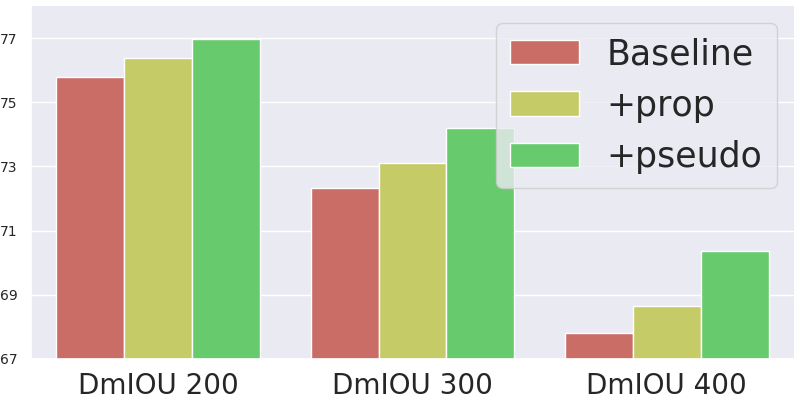
\includegraphics[height=0.4\linewidth]{figures/dmiou.png}
% }%
% {%
%     \vspace{-0.3em}%
%     \caption{\small Measuring the improvement on Distance based mIoU by training on pseudo-labels.}
%     \label{fig: figure-label}
% }%
% \killfloatstyle\ttabbox[\Xhsize]
% {%
%     \begin{tabular}[t]{llcc}
%         \toprule
%         \multicolumn{2}{l}{} & mIOU & $\text{\tiny DmIOU}_{200}$ \\
%         \midrule
%         \multicolumn{2}{l}{Baseline} &  &\\
%         \multicolumn{2}{l}{Baseline + SDC} & &\\
%         \multicolumn{2}{l}{Baseline + LID} & & \\
%         \multicolumn{2}{l}{Baseline + GT} & & \\
%         \bottomrule
%     \end{tabular}
% }%
% {%
%     \caption{\small Benefit of training with pseudo-labels on ApolloScape Dataset}\label{tab: table-label}
% }%
% \end{floatrow}

% % \caption{\small \emph{Left:} The sequence error for SVHN multi-digit recognition
% % on crops of $64\times 64$ pixels (64px), and inflated crops of $128 \times 128$
% % (128px) which include more background. \textsuperscript{*}The best reported
% % result from \cite{Ba14} uses model averagin}
% % % }}%
% \vspace{-1em}
% \end{figure}

\begin{table}[t]
    \centering
    \caption{ We show the benefit of training with our pseudo-labels. We also show the benefit of modelling label uncertainty. In the above table,  $D_{\hat{L}seq}$ contains propagated labels and $D_{\hat{L}ps}$ contains pseudo-semantic labels (refer Section~\ref{subsec-alea}).
    }\label{tab_main_ablation}
    \begin{tabular}{llcc}
\toprule
\multicolumn{2}{c}{Dataset}& Loss & mean IOU  \\
\midrule
\multicolumn{2}{l}{$D_L$} & C.E. & 77.62\\
\multicolumn{2}{l}{$D_L$ + \cite{nvidia_cvpr19} ($\pm 2,4,6,8$)}& RLL &77.82  \\
\multicolumn{2}{l}{$D_L$ + Ours ($\pm [2,4,6,8])$}&$\mathtt{UAT}$ & 78.45  \\
\midrule
\multicolumn{2}{l}{$D_L$ + GT($\pm [2,4,6,8])$}& \cite{gal_main} & 77.82  \\
\bottomrule
    \end{tabular}
\end{table}
 
% \begin{table}[t]
% \begin{center}\small
% % \setlength{\tabcolsep}{3pt}
% \begin{tabular}[t]{lccc}
% %%%%%% Title row starts here
% \\
% % Temporary header Graph would be better! TBD
% \toprule
% \multicolumn{1}{l}{} & $\text{{\tiny DmIOU}}_{200}$ & $\text{\tiny DmIOU}_{300}$ & $\text{\tiny DmIOU}_{200}$ \\
% \midrule
% \multicolumn{1}{l}{Baseline} & 75.79 & 72.32 & 67.80\\
% \multicolumn{1}{l}{+ prop} & 76.37 & 73.10 & 68.66 \\
% \midrule
% \multicolumn{1}{l}{+pseudo} & 76.37 & 73.10 & 68.66 \\
% \bottomrule
% \end{tabular}
% \qquad\qquad \qquad\qquad
% % \hspace{-2em}
% % \vtop{
% % \vspace{-1em}
% % \hbox{
% % 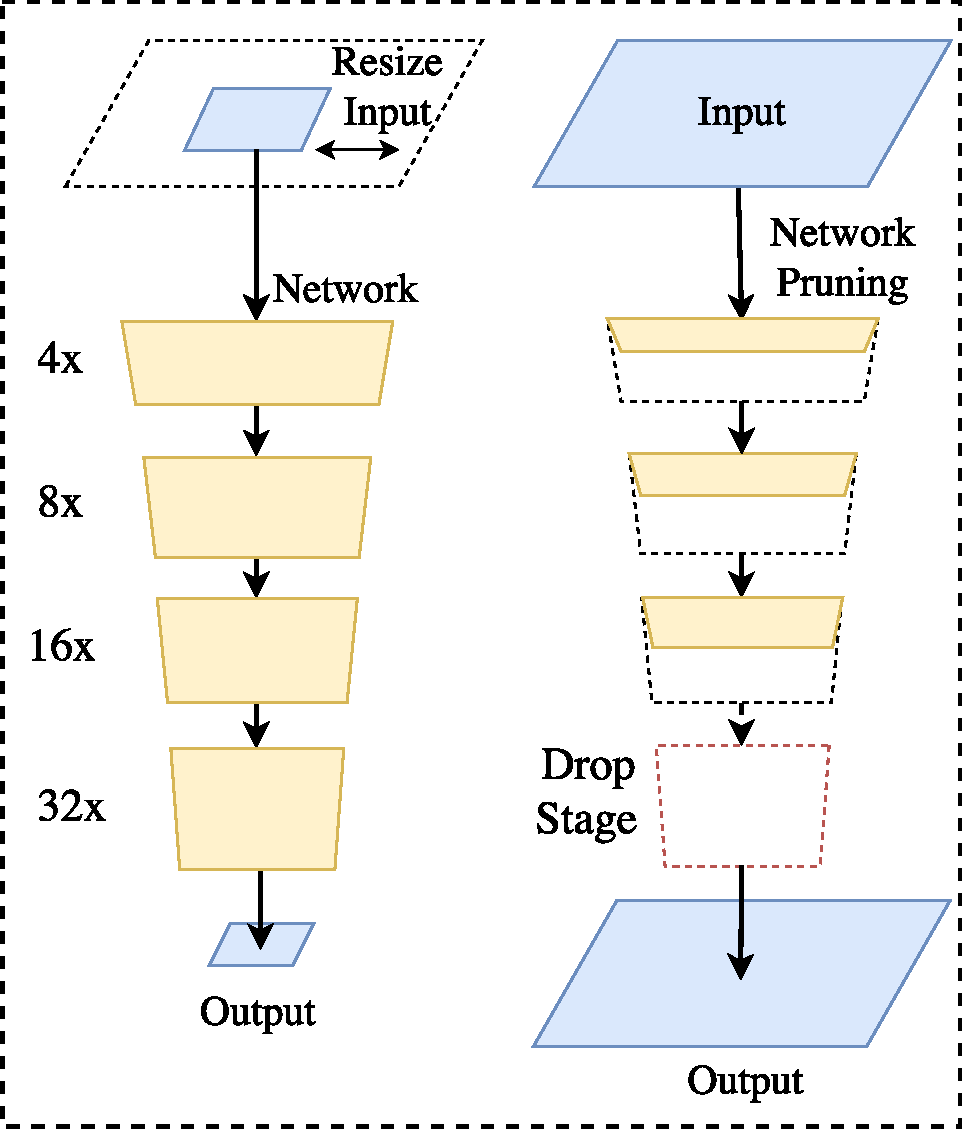
\includegraphics[width=0.6\textwidth]{figures/input_model.pdf}
% \begin{tabular}[t]{llcc}
% %%%%%% Title row starts here
% \toprule
% \multicolumn{2}{l}{} & mIOU & $\text{\tiny DmIOU}_{200}$ \\
% \midrule
% \multicolumn{2}{l}{Baseline} &  &\\
% \multicolumn{2}{l}{Baseline + SDC} & &\\
% \multicolumn{2}{l}{Baseline + LID} & & \\
% \multicolumn{2}{l}{Baseline + GT} & & \\
% \bottomrule
% \end{tabular}

% % }}%
% \end{center}
% \caption{\small \emph{Left:} The sequence error for SVHN multi-digit recognition
% on crops of $64\times 64$ pixels (64px), and inflated crops of $128 \times 128$
% (128px) which include more background. \textsuperscript{*}The best reported
% result from \cite{Ba14} uses model averagin}
% \label{table:svhn}
% \end{table}

% \let\clearpage\relax
% 
% \begin{table}[t]

% % \caption{\small \emph{Left:} The sequence error for SVHN multi-digit recognition
% % on crops of $64\times 64$ pixels (64px), and inflated crops of $128 \times 128$
% % (128px) which include more background. \textsuperscript{*}The best reported
% % result from \cite{Ba14} uses model averagin}
% % % }}%
% \vspace{-1em}
% \end{table}


\begin{table}[t]
\begin{center}\small
% \setlength{\tabcolsep}{3pt}
    \begin{tabular}{lc}
        \toprule
        \multicolumn{1}{c}{Method}& mean IOU  \\
        \midrule
        % DenseASPP \cite{Yang2018DenseASPP}&  80.6 \\
        % SPG  \cite{Cheng2019SPGNet}  &     $81.1$        \\
        % DANet  \cite{Fu2018DANet} &     $81.5$        \\
        HRNetv2  \cite{Sun2019HRNet}     &     $81.8$        \\
        EMANet  \cite{Li2019EMANet}&     $81.9$        \\
        ACNet \cite{Fu2019ACNet}&  \secbest{82.3}        \\
        \midrule
        Our Baseline  &     80.9        \\
        Ours WRP + UAT  &     \best{82.3}        \\
        \bottomrule
    \end{tabular}
\qquad\qquad \qquad\qquad
% \hspace{-2em}
% \vtop{
% \vspace{-1em}
% \hbox{
% 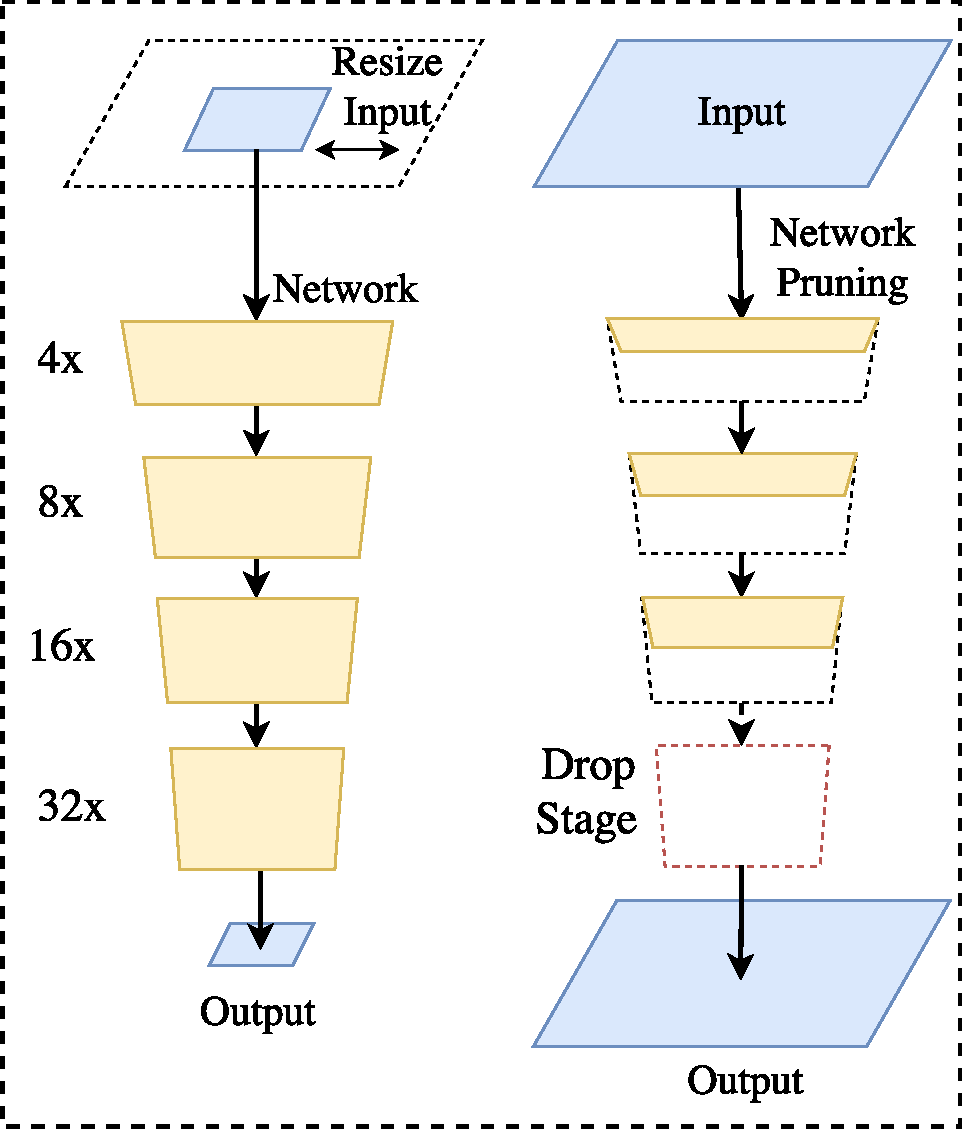
\includegraphics[width=0.6\textwidth]{figures/input_model.pdf}
    \begin{tabular}{llcc}
        \toprule
        \multicolumn{2}{c}{Dataset}& Loss & mean IOU  \\
        \midrule
        \multicolumn{2}{l}{$D_L$} & C.E. & 77.62\\
        \multicolumn{2}{l}{$D_L$ + \cite{nvidia_cvpr19} ($\pm 2,4,6,8$)}& RLL &77.82  \\
        \multicolumn{2}{l}{$D_L$ + Ours ($\pm [2,4,6,8])$}&$\mathtt{UAT}$ & 78.45  \\
        \midrule
        \multicolumn{2}{l}{$D_L$ + GT($\pm [2,4,6,8])$}& \cite{gal_main} & 77.82  \\
        \bottomrule
    \end{tabular}

% }}%
\end{center}
\caption{\small \emph{Left:} The sequence error for SVHN multi-digit recognition
on crops of $64\times 64$ pixels (64px), and inflated crops of $128 \times 128$
(128px) which include more background. \textsuperscript{*}The best reported
result from \cite{Ba14} uses model averagin}
\label{table:svhn}
\end{table}

% Can also have just one table


To benefit from propagated data, we find it essential to include propagated samples from multiple timesteps. Following~\cite{lp_eccv}, for each label in $D_L$, we include propagated labels at timesteps $t \pm p$ where $p \in \{2,4,6,8\}$ from $D_{\hat{L}seq}$. Furthermore, we include pseudo-labelling on the \texttt{train\_extra} subset $D_{\hat{L}ps}$ as well. The results are shown in Table~\ref{tab_main_ablation}. The propagated labels, when used with the \emph{Uncertainty-Aware Training} (UAT), enable us to boost the performance $0.49$ mIoU. The performance is further boosted by $0.47$ mIOU when $D_{\hat{L}ps}$ is used as well. Note how UAT plays a crucial role in increasing performance in the presence of propagated labels.
%   While simply adding the generated labels is found to be useful, the improvement is constraint by the noise in these labels. Once we introduce the uncertainty based learning (section~\ref{subsec-alea}), we are able to boost the result further. 

Finally, using the same method, we show that it is able to improve the \textit{state-of-the-art} on Cityscapes (when training with fine labels only). Table~\ref{} shows the improvement by training with our method. We observe that in the presence of coarse labels, and Mapillary Vistas pretraining~\cite{mapillary}, the benefits of label propagation are not clear (shown in supplementary). This is expected as label propagation cannot be performed for the coarse labels and the Mapillary Vistas dataset and hence, in the presence of those labels, propagation is performed for only $\sim$ 10\% of the entire dataset.

% \textbf{Stronger Metric}: Following~\cite{gated_iccv2019}, we also evaluate the distance-based mIoU, which measures performance on objects far away from the camera, which is much harder. The results are shown in Table~\ref{}, showing that the generated labels significantly help with objects further away.
% As the performance in Cityscapes dataset is found to be saturating, we find mIOU to be a insufficient metric to show improvements in performance. 
%Table~\ref{} compares our results with previous methods and show that the 0.6 \% improvement in mIOU translates to significant improvement in segmentation of objects far from the camera. 


\textbf{Evaluation on ApolloScape}: In Table~\ref{} we show the benefit of training with propagated labels and the uncertainty-aware training regime on Apolloscape dataset. %We find a improvment of x\% mIOU over the baseline using our labels and uncertainty based training.

\textbf{Modelling Label Noise with Uncertainty}: We demonstrate that the uncertainty estimates are able to model the noise in the data-generation process. Figure~\ref{} shows the precision-recall curves between the generated label $D_{\hat{L}seq}$ and manually annotated labels $D_{Lseq}$ on ApolloScape. % They show that the uncertainty is higher for noisy propagated labels. % label quality improves by removing labels with uncertainty larger than various percentile thresholds.



% What are the experiements: 
% 1) Apolloscapes  ppa/miou graph + examples on right. => By 25th
% 2) Previous dont work + uncertainty plot. 
% 2) Ablation ours Big table
% 3) Big table test on Cityscapes. Fine Only with All. =. End moment
% 4) L:Apolloscapes table mIOU. R: Finer metrics on Cityscapes.  = L: 27th, R: 23rd

% Supplementary: 
% 1) Failure all put in nvidia
% 2) All put in ours (val and test?)
% 3) propagation ablations.
% 4) Proof
% 5) Video
% 6) More image examples. 
